\section{Übertragungsmedien}
    \paragraph{Signale}
    \begin{formula}{Ausbreitungsgeschwindigkeit}
        $C_{Medium} = 200'000 km/s \approx 2/3 c_0$

        \vspace{1mm}

        {\small $c_0$: Lichtgeschwindigkeit im Vakuum ($3 \cdot 10^8 m/s$)}
    \end{formula}

    \begin{formula}{Signaldämpfung} Leistungsabnahme auf Übertragungsstrecke
        
        \vspace{1mm}
        
        $Signaldämpfung[dB] = 10 \cdot log (\frac{\textcolor{red}{P_1}}{\textcolor{red}{P_2}}) = 10 \cdot log((\frac{\textcolor{blue}{U_1}}{\textcolor{blue}{U_2}})^2) = 20 \cdot log(\frac{\textcolor{blue}{U_1}}{\textcolor{blue}{U_2}})$

        \vspace{1mm}

        {\small \textcolor{red}{$P_1$}: Anfangsleistung, \textcolor{red}{$P_2$}: Leistung am Ende der Strecke\\
        \textcolor{blue}{$U_1$}: Anfangsspannung, \textcolor{blue}{$U_2$}: Spannung am Ende $\Rightarrow$ \textcolor{blue}{Amplitude des Signals}}

        \includegraphics[width=1\linewidth]{images/Signaldämpfung.png}\\
        {\small Halbierung der Leistung entspricht ca. 3dB}
    \end{formula}    

    \begin{formula}{Signal to Noise Ratio} 
        $SNR_{dB} = 20 \cdot log(\frac{\textcolor{blue}{U_Signal}}{\textcolor{blue}{U_Störung}})$
    \end{formula}

    \begin{definition}{Dämpfungsbelag}
        $\text{Dämpfungsbelag } = \frac{Dämpfung_{dB}}{Länge_{m}} \cdot 100$

        \vspace{1mm}

        {\small Dämpfung pro Distanz - dB pro 100m (Coax < TP CAT7 < TP CAT3)}
    \end{definition}

    \begin{concept}{Maximale Leistungslänge} $L_{max} = \frac{SNR_{min}}{Dämpfungsbelag}$

        \vspace{1mm}

        {\small $SNR_{min}$: Minimales benötigtes SNR für korrekte Datenübertragung}

        \vspace{1mm}

        \begin{itemize}
            \item tiefere Bitrate $\rightarrow$ grössere Distanzen können erreicht werden
            \item Die Bandbreite (Frequenz) ist abhängig zum Dämpfungsbelag.
            \item höhere Kabelkategorien haben bessere Schirmung $\rightarrow$ tolerieren höhere Dämpfung
        \end{itemize}
    \end{concept}

    

    \paragraph{Kabeltypen}
    \begin{concept}{Overview}
        \begin{itemize}
            \item Koaxialkabel: Geeignet für hochfrequente Signale
            \item Twinaxialkabel: Hoher Schutz (double koax)
            \item Twisted Pair (TP): Häufig im Einsatz (Shielded/Unshielded)
            \item Glasfaser: Hohe Bandbreite, resistent, Geringe Dämpfung - aber Dispersion (Lichtgeschwindigkeit abhängig von Wellenlänge)
                \begin{itemize}
                    \item Multimode, Singlemode (besser)
                \end{itemize}
        \end{itemize}        
    \end{concept}

    \begin{definition}{Paarsymmetrische Kabel (Twisted Pair)}
        \begin{itemize}
            \item Schirmeigenschaften
            \begin{itemize}
                \item Drahtgeflecht: niederfrequente Einstreuungen
                \item metallisch beschichtete Folien: hochfrequente Störungen
            \end{itemize}
            \item Bezeichnungsschema ISO/IEC 11801\\
            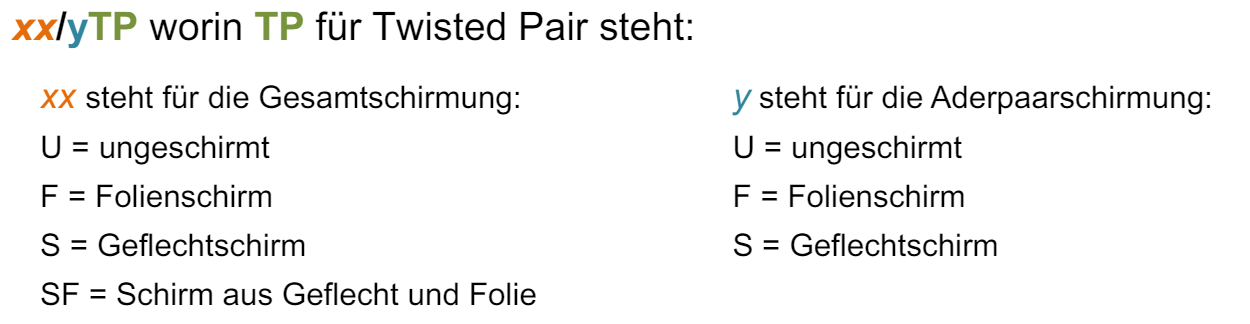
\includegraphics[width=\linewidth]{images/STP_Schirmeigenschaften.png}
        \end{itemize}
        Behebung von Störungen (crosstalk):
        \begin{itemize}
            \item Kapazitiv: Komplementäres Signal, elektrisch leitenden Schirm
            \item Induktiv: Verdrillte Aderpaare
        \end{itemize}
    \end{definition}

    

    
        
    